The bare-minimum multirotor remote-piloted aerial system (RPAS) consists of a propulsion system, flight controller, speed controllers, battery/fuel, and sensor systems.

\subsubsection{Multirotor Configuration}

A multirotor RPAS (MRPAS) has several common configurations, a tricopter, a quadcopter, and a hexacopter.

\begin{figure}[H]
    \centering
    \begin{subfigure}[b]{0.3\textwidth}
        \centering
        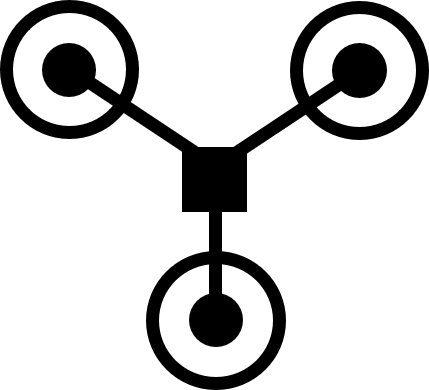
\includegraphics[scale=0.4]{img/drone_yconfig}
        \caption{Tricopter Y-Configuration}
        \label{fig:tricopter-y}
    \end{subfigure}
    ~
    \begin{subfigure}[b]{0.3\textwidth}
        \centering
        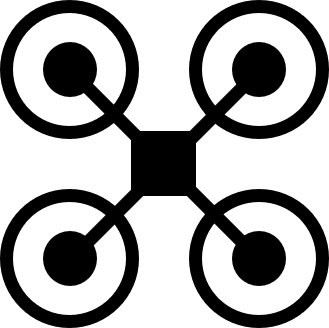
\includegraphics[scale=0.4]{img/drone_xconfig}
        \caption{Quadcopter X-Configuration}
        \label{fig:quadcopter-x}
    \end{subfigure}
    ~
    \begin{subfigure}[b]{0.3\textwidth}
        \centering
        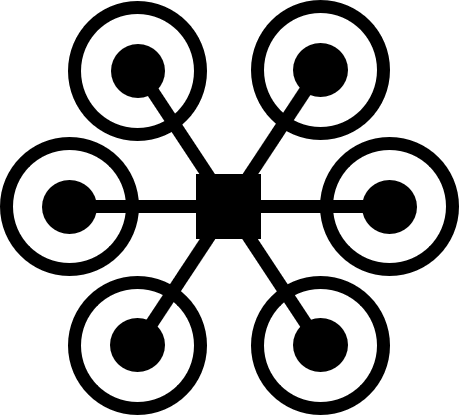
\includegraphics[scale=0.4]{img/drone_hexconfig}
        \caption{Hexcopter X-Configuration}
        \label{fig:hexcopter-x}
    \end{subfigure}
    
    \caption{Multirotor RPAS configurations}
    \label{fig:rpas_configs}
\end{figure}

\textbf{Tricopter: }The benefit of a tricopter, as represented in figure \ref{fig:tricopter-y} comes from its fewer required motors and speed controllers,
which means less power draw required to sustain flight. Each arm that is supporting each motor is also wider, at 120 
degrees. This makes the motors and arms of the MRPAS less visible from the mounted camera's point of view. 
However, the downside of a tricopter is that there exists asymmetry of motor torque (Figure \ref{fig:tricopter-y-t}) since 
there is an odd number of motors. An additional servo motor is required to control the tail motor which 
complicates the control algorithms for self-stabilizing flight.

\begin{figure}[H]
    \centering
    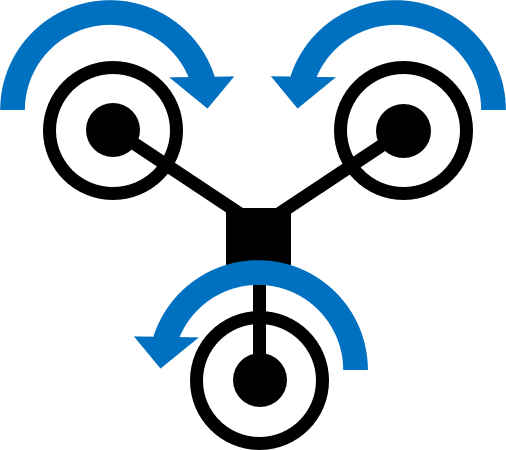
\includegraphics[scale=0.4]{img/drone_yconfigt}
    \caption{Tricopter Y-configuration has non-zero resultant motor torque}
    \label{fig:tricopter-y-t}
\end{figure}

\textbf{Quadcopter X: }
The quadcopter is the most common configuration in consumer multirotor products. The quadcopter is more stable than a tricopter because a quadcopter configuration utilizes four motors (Figure \ref{fig:quadcopter-x-t}). Two of the motors spins  
clockwise and the other two spins counter-clockwise, effectively cancel each other’s undesired torque. 
Applying the same power into each motor allows the MRPAS to hover in place. We can perform 6 degree-of-freedom (DOF) movements by changing a combination of differential thrust to each motor (Figure \ref{fig:rpas_6dof}).

\begin{figure}[H]
    \centering
    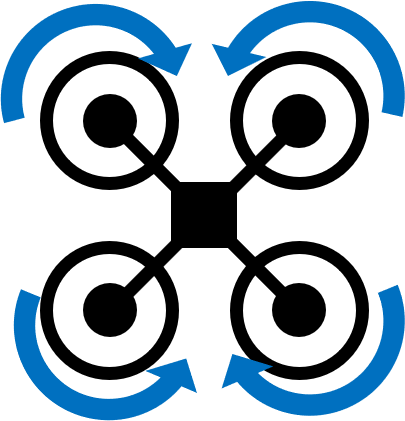
\includegraphics[scale=0.4]{img/drone_xconfigt}
    \caption{Quadcopter X-configuration has zero resultant motor torque}
    \label{fig:quadcopter-x-t}
\end{figure}

\begin{figure}[H]
    \centering
    \begin{subfigure}[b]{0.3\textwidth}
        \centering
        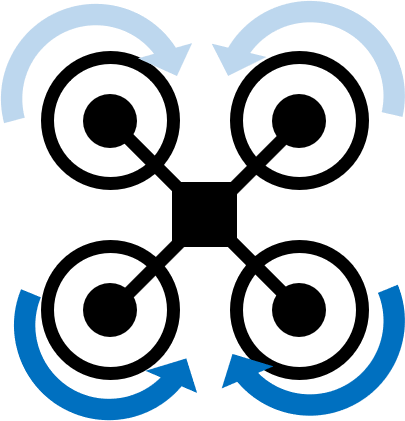
\includegraphics[scale=0.4]{img/drone_x_pitch}
        \caption{Pitch forward}
        \label{fig:x-pitch}
    \end{subfigure}
    ~
    \begin{subfigure}[b]{0.3\textwidth}
        \centering
        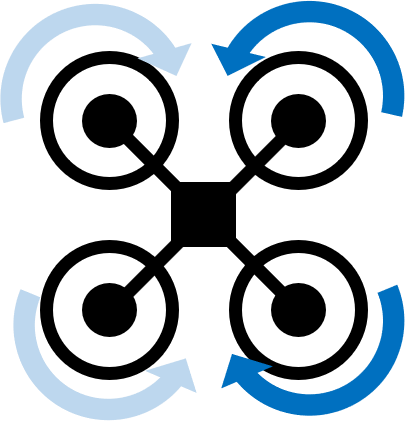
\includegraphics[scale=0.4]{img/drone_x_roll}
        \caption{Roll left}
        \label{fig:x-roll}
    \end{subfigure}
    ~
    \begin{subfigure}[b]{0.3\textwidth}
        \centering
        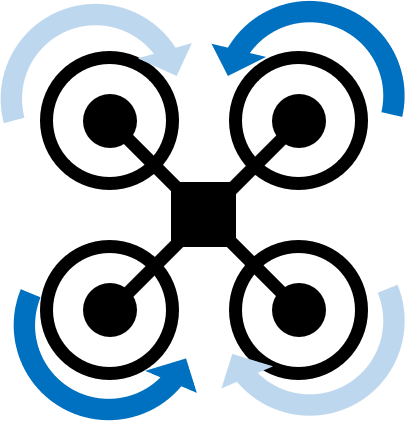
\includegraphics[scale=0.4]{img/drone_x_yaw}
        \caption{Yaw left}
        \label{fig:x-yaw}
    \end{subfigure}
    
    \caption{Using differential thrust to obtain 6-DOF movement. }
    \label{fig:rpas_6dof}
\end{figure}

\textbf{Hexacopter X: }
The hexacopter has all the stability benefits of a copter. In addition, the hexacopter configuration also 
offers redundancy. Up to 2 motors can fail and the MRPAS could still land safely. Due to the added 
propulsion systems (50\% more than the quadcopter configuration), hexacopter can generally lift more 
payload than quadcopters. The downside is that hexacopter configuration builds are more expensive to build, 
operate, and maintain. Upon a crash, due to hexacopter MRPASs extended size and weight cause more injuries 
or collateral damage to nearby equipment.

We choose to pursue with a quadcopter configuration. 
The payload is not too heavy, our target maximum payload weight is less than 500 g (\textbf{NF.DR.1}). The quadcopter configuration is also the most balanced in terms of trade-off between cost and reliability. 

\subsubsection{Air Frame}\label{section:air-frame}

The most common frames available for sale comes in 450 mm motor to motor diagonal span (MMDS). However, 
350mm is also common amongst consumer products such as DJI Phantom. The problem with 350 mm is that it will 
constrain our ability to mount larger hardware such as the computing platform. The 350 mm also limits 
propeller size. On the other hand, the largest quadcopter configuration has an MMDS of 650 mm or 1000 mm 
for extremely large payload capacity. However, these are more commonly used for industrial or military 
applications.

\begin{figure}[H]
    \centering
    \begin{subfigure}[b]{0.33\textwidth}
        \centering
        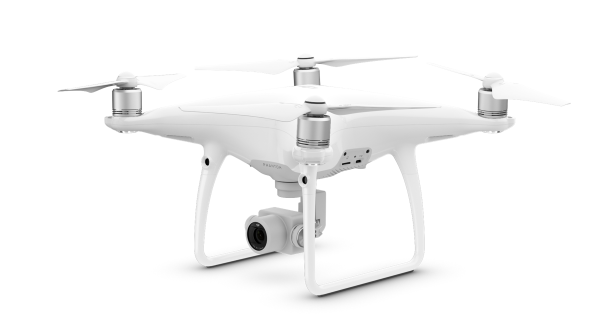
\includegraphics[width=\textwidth]{img/djiphantom4}
        \caption{DJI Phantom 4 (350 mm)}
    \end{subfigure}
    ~
    \begin{subfigure}[b]{0.33\textwidth}
        \centering
        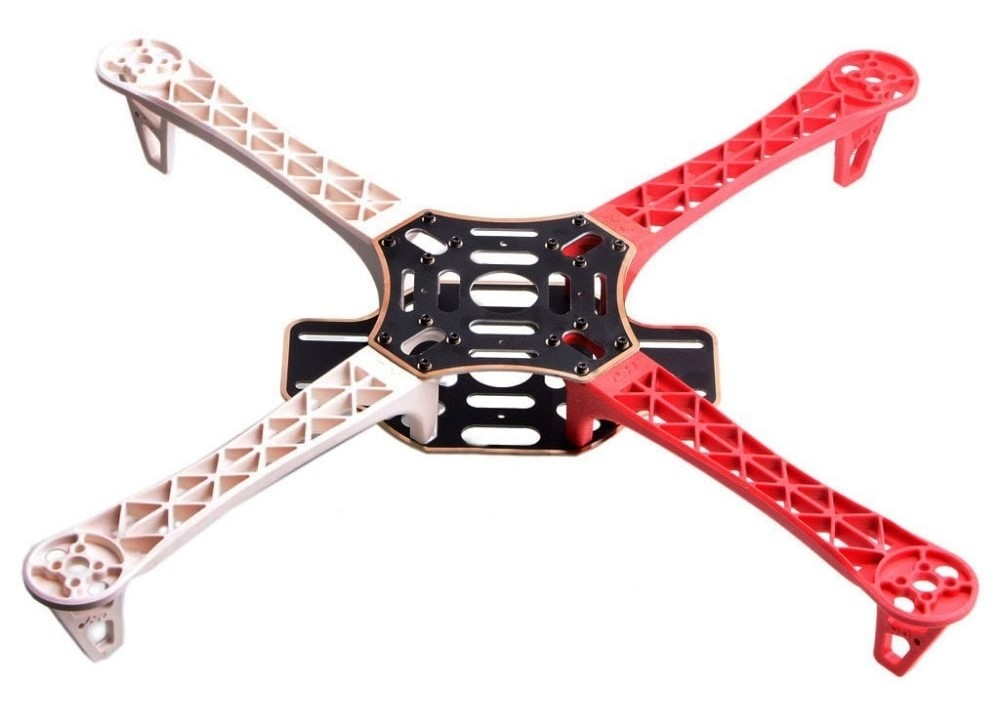
\includegraphics[width=\textwidth]{img/f450frame}
        \caption{Generic DIY frame kit (450 mm)}
    \end{subfigure}
    ~
    \begin{subfigure}[b]{0.33\textwidth}
        \centering
        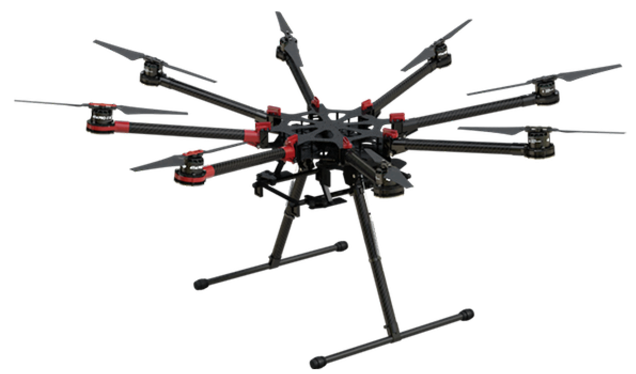
\includegraphics[width=\textwidth]{img/djis1000}
        \caption{DJI Spreadwings S1000 (1000 mm)}
    \end{subfigure}
    
    \caption{Various air frame sizing options. }
    \label{fig:}
\end{figure}

We choose a frame size of 450 mm MMDS that has a good balance between portability and capability. The frame 
can accommodate larger propellers (see in later section XX in propeller size). Furthermore 450 mm are the 
most abundant size on the market for frames because of their versatility and therefore is also less costly 
and easy to repair/replace.

Currently, the \textit{Upgrade F450} for CA\$30.00 and \textit{Diatone Q450} for CA\$20.00 from Banggood are appealing options. They weigh between 300 g to 410 g which is acceptable.

\subsubsection{Propulsion System}

Propulsion system covers the majority of the RPAS parts list and will determine the flight performance of the RPAS. 

\paragraph{Motor Type}

The MRPAs is electrically powered with a battery (DC). Thus, we have two options for motors: DC brushed 
motors and DC brushless motors.

Brushed motors use mechanical brushes in contact with rotor’s commutator to switch polarity to sustain a 
constant rotation, whereas the brushless motors use electronic controllers to switch the polarity in the 
rotor electrically. 

For the flight applications, we choose the brushless DC (BLDC) motors for their extended usable life time. 
BLDC motors are also much more efficient than brushed motors because we do not have to mechanically swap 
the polarity in the motor, which results in excess friction, heat, and potential sparking.

BLDC motors are further broken down into two types: in-runner and out-runner. The in-runner have the rotor 
on the inside and the out-runner has the rotor on the outside. We choose out-runner because they’re 
commonly used for multirotor RPAS. The out-runner also comes with benefits: because the rotor is on the 
outside, heat dissipation is significantly more efficient. Since the rotating mass is further from the 
center of rotation for an out-runner, the rotational inertia helps stabilizing the angular momentum of the 
rotor. Of course, this means that the out-runner has a slower spin-up time than the in-runner, but for a 
multirotor RPAS typically operating in stabilized flight and hover, the agility of an in-runner is not 
practical.

\paragraph{Motor Size and Speed}\label{section:motor-speed}

All BLDC out-runner motors have the same height, and on product pages they are often given the code 22XX to denote their stator size. The design parameter is the radius (XX on the product code). Typically, the larger the stator (radius), the slower it spins given the same voltage. This is a linear relationship described by the motor parameter kV:

$$
\omega_{\mathrm{RPM}} = \mathrm{kV} \times \mathrm{Voltage}
$$

The kV constant is inversely proportional to another motor constant, kT, which models the linear relationship between current and torque:

$$
\tau = \mathrm{kT} \times \mathrm{Current}
$$

The inverse relationship can be shown by equating electrical power into the motor and mechanical power produced by the motor:

$$
\tau\omega_{\mathrm{RPM}} = \mathrm{kV}\mathrm{kT}\times VI
$$

By constraining the electrical power, we can make trade-off between torque and rotation speed.
Air resistance, or “drag” is proportional to speed of an object squared therefore the power required to 
lift increases non-linearly to the force output. As seen in the test data obtained from one manufacturer’s 
datasheet below, using the same propellers we see an increased thrust output from increased voltage (and 
thus current). However, the efficiency, typically measured in g/W decreases. 

Below is a sample set of thrust output using a SunnySky X2216 1250 kV motor using 9.0 inch 5.0\si{\degree} pitch and 10.0 inch 4.7\si{\degree} pitch propellers obtained from vendor website \cite{sunnysky-2216}. 

\begin{table}[H]
    \centering
    \caption{Sample motor test data demonstrates decrease in g/W efficiency as thrust output increases.}
    \label{table:sunnyskyx2216-table}

    \begin{tabular}{lrrrrr}

    \hline
    \textbf{Propeller} & \textbf{Voltage} & \textbf{Current} & \textbf{Pull}  & \textbf{Power Consumption} & \textbf{Efficiency}\\
    & [V] & [A] & [g] & [W] & [g/W] \\
    \hline
     & 10.0 & 16.4 & 940 & 164 & 5.73 \\
    9050 & 11.0 & 19.5 & 1050 & 215 & 4.89 \\
     & 12.0 & 21.5 & 1250 & 258 & 4.84 \\
    \hline
     & 10.0 & 23.5 & 1200 & 235 & 5.10 \\
    1047 & 11.0 & 26.5 & 1350 & 372 & 3.63 \\
     & 12.0 & 30.2 & 1520 & 363 & 4.19 \\
    \hline

    \end{tabular} 
\end{table}

Therefore, it makes sense that we choose larger motors with relatively lower kV constants. Slower motors 
are also safer since there is less angular momentum of the blades. Motors with 800 kV to 1300 kV are 
suitable for our applications and achieve reasonable thrust output with adequate efficiency. 2212, 2214, 
and 2216 stator sizes are suitable in this range of kV.

\paragraph{Propeller Material}

Common RPAS propellers are constructed in either plastic or carbon composite. Plastic is cheap, abundant, 
and relatively flexible. But due to their cheapness, their manufacturing is not as precise which leads to 
aerodynamic inefficiencies. Plastic propellers often require balancing where tape is applied to one of the 
blades such that the weight is balanced---minimizing vibrations. Carbon composite propellers, such as 
carbon fibre blades, are extremely light and subsequently much more expensive. But the carbon composite 
propellers have micro-meter precision manufacturing which provides top efficiency. Carbon composite 
propellers are not flexible and extremely tough. It is more dangerous for persons to be near spinning 
carbon composite propellers due to its sharpness and toughness, and could lead to serious injuries or death.

Due to budget constraint and safety concerns, we choose plastic propellers.

\paragraph{Propeller Size and Pitch}

\textbf{Notation: } Propeller size and pitch is commonly denoted by RRYY where RR is the propeller diameter in inches, and YY is the propeller pitch in degrees. (9050 denotes a propeller with 9 inch diameter, and 5.0 degrees of pitch; 1045 denotes a propeller with 10 inch diameter, and 4.5 degrees of pitch).

\begin{figure}[H]
    \centering
    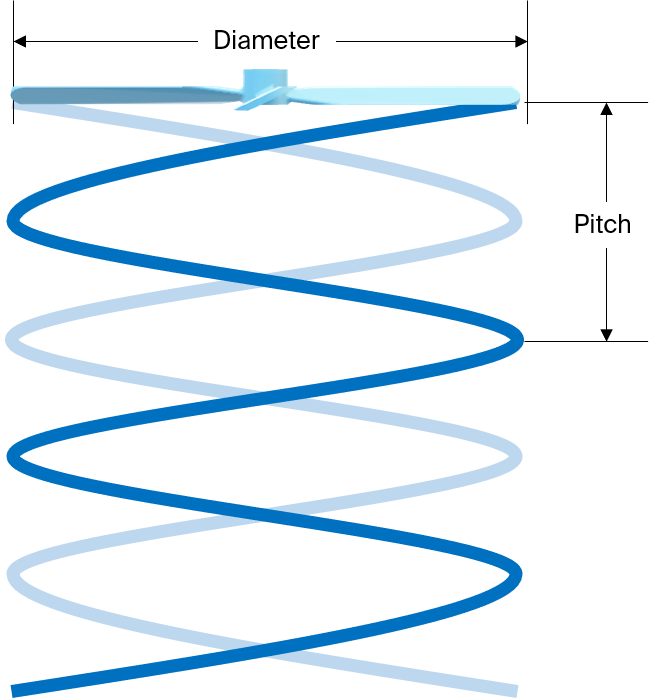
\includegraphics[scale=0.5]{img/proppitch}
    \caption{Diameter and pitch parameters of a propeller}
    \label{fig:propeller}
\end{figure}

To obtain maximum thrust with low speed (low speed is more desirable, as mentioned in Section \ref{section:motor-speed}), we want to choose the biggest possible propeller diameter.

\begin{figure}[H]
    \centering
    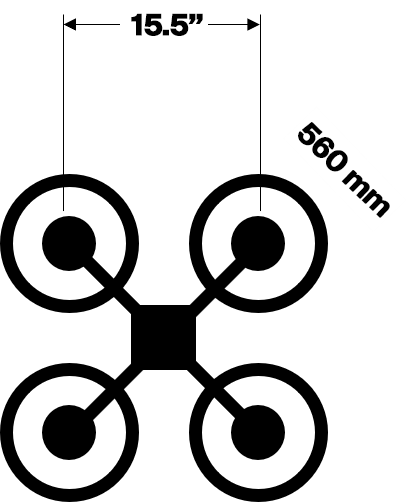
\includegraphics[scale=0.5]{img/framepropsize}
    \caption{Maximum propeller size is determined by the size of the frame.}
    \label{fig:framepropsize}
\end{figure}

As mentioned in Section \ref{section:air-frame}, we choose the 450 mm frames, which means that the motor to motor 
adjacent span (MMAS) is about 12.5 inches. It is safe to provide 1 inch of clearance between propellers, 
therefore the ideal size of propellers we choose is 10 or 11 inches.

Mentioned in  Section \ref{section:motor-speed}, we choose low-speed motors for their efficiencies. And recall that 
given the same power: a slow-speed motor provides inversely proportional high-torque, we choose propellers 
with relatively high pitch (between 3 to 5 degrees) to take advantage of the high-torque output and 
maximize thrust output.

Here is a list of desirable propeller size and pitches: 1030, 1045, 1130, 1145.

\paragraph{Speed Controllers}

The electronic speed controller (ESC) controls the voltage and current supplied to a BLDC motor. All ESCs 
function identically and the design parameters are size/weight, rating, efficiency, and cost.

As shown in Table \label{table:sunnyskyx2216-table} the typical maximum current draw is about 30 A. For a 
safety margin of 10 A, we decided to select ESCs with maximum rating of 40 A. All of below are appealing 
options:

\begin{table}[H]
    \centering
    \caption{ESC Purchasing Options}
    \label{table:esc-table}

    \begin{tabular}{lrrrll}

    \hline
    \textbf{ESC} & \textbf{Rating} & \textbf{Weight} & \textbf{Price}  & & \textbf{Vendor}\\
    & [A] & [g] & [CA\$] & & \\
    \hline
    HAKRC BLHeli Dshot1200 & 35 & 7  & 40.00 & per 4 & Banggood\\
    Racestart RS30A Lite & 30 & 6  & 40.00 & per 4 & Banggood\\
    Racestart SPROG X DShot600 & 35 & 4  & 30.00 & per 4 & Banggood\\
    Skystars Talon32 & 40 & 7  & 12.00 & per 1 & Banggood\\
    \hline

    \end{tabular} 
\end{table}

\subsubsection{Flight Controller}

Flight controller (FC) comes in different tiers differentiated by their price and features. 

The cheapest FC typically only has the bare-minimum features for flight such as accelerometers and 
self-hover functions. These flight controllers are typically designed for acrobatic or basic VLOS 
flying and typically cost CA\$20 to CA\$50. The firmware that runs on these FC are typically 
open-source but nonetheless user-friendly and easily-programmable. Below is a list of FC that falls 
under this tier:

\begin{itemize}[noitemsep,topsep=0pt, parsep=4pt, partopsep=0pt]
    \item F1, F3, F4, F7 FC are minimal in weight and footprint; they are ideal for light-weight operations.\cite{f1fc}
    \item KK 2.15 FC features a built-in display on the board, allowing quick access to flight settings without the need to connect to a computer for reprogramming.
    \item Naze32 FC is reliable with auto-tuning PIDs.
    \item CC3D FC is reliable with auto-tuning PIDs.
\end{itemize}

The next tier of FC have more advanced features such as GPS-hold, autonomous flight, anto-land, 
telemetry, etc. They are designed for more advanced operation. These FCs are more expensive costing 
CA\$50 to CA\$200. However, these FCs have excellent after-sale support for their respective 
manufacturers and documentation is better. The FCs are also rigorously tested in the industry. Along 
with frequent manufacturer firmware updates, the mid-tier FCs are more liable. The downside is that 
they are typically heavier with weather-resistant enclosures and takes up a much larger footprint. 
Below is a list of mid-tier FCs:

\begin{itemize}[noitemsep,topsep=0pt, parsep=4pt, partopsep=0pt]
    \item ArduPilot APM 2.8 is a flight controller using Arduino Mega and supports GPS and telemetry.
    \item Pixhawk PX4 Autopilot features pre-programmable autonomous operations.
    \item DJI Naza M Lite.
\end{itemize}

For the applications we need, we choose ArduPilot APM 2.8 as it is the most flexible option with advanced features at a reasonable price of CA\$75.00. Additionally due to of the low-cost of low-tier FCs, we will also purchase one of Naze32 or CC3D FC as a back-up.

\subsubsection{Radio Systems}

The minimum number of channels required to fly a drone is 4. One for each control: throttle, yaw, 
pitch, and roll. For that reason, we opt for the cheapest radio transmitter (TX) and receiver  (RX) 
combo we find from online vendors. 
The FlySky-FS i6 2.4GHz 6-Channel TX and RX bundle is ideal for our application for its lowcost.
According to FlySky-FS i6 datasheet\cite{flyskyi6} , the radio frequency (RF) peak power is below 20 dBm and still achieves maximum control range of 500 m, and thus satisfies the requirement \textbf{NF.DR.5}.

\subsubsection{Battery}

We choose lithium polymer (Li-Po) batteries because they have the highest energy density (highest 
capacity to weight ratio), and thus perfect for high-power, low-weight applications such as flying. 

Li-Po batteries have mainly three design parameters: configuration, capacity, and discharge rating. 
Configuration is how the Li-Po batteries are wired up: a single-cell Li-Po battery can provide a 
nominal voltage of 3.7 V due to its electrochemistry. Multiple cells can be put in series and the 
voltage adds up: 2S (2 cells in series) batteries have 7.4 V output, 3S batteries have 11.1 V output,
 and 4S batteries have 14.8 V output.

Battery capacity is measured in watt-hours (Wh) or milli-amp-hours (mAh) which is power multiplied by time. A 20 Wh battery can output 20 W for 1 hour. Multiple cells of batteries can be put in parallel and the capacity adds up. 4S2P batteries have 14.8 V ouput but has double the capacity than 4S batteries.

Lastly, the discharge rating is denoted by “C” and indicates the maximum discharge current. A 1,000 
mAh battery with a discharge rating of 20 C can discharge a maximum of 1.0 A $\times$ 20 C = 20 A.

We choose the design parameters for the battery after we have consolidated on rest of the parts for the RPAS since batteries comes in many sizes and configurations, and allows more flexibility.
